\documentclass[a4paper,twoside,15pt]{book}
\usepackage[utf8]{inputenc}
\oddsidemargin=1cm
\evensidemargin=1cm
\addtolength{\textwidth}{1in}
\addtolength{\voffset}{-5pt}

\title{Moravia Microsystems - The Business Plan}
\author{Martin Ošmera <martin.osmera@gmail.com>, Erik Chalupa <xchalu10@stud.fit.vutbr.cz>, Martin Madron <pomerange@seznam.cz>}

\newcommand{\mysubject}{Moravia Microsystems, the company business plan.}
\newcommand{\mykeywords}{Moravia Microsystems}

\usepackage[T1]{fontenc}
\usepackage{float}
\usepackage{graphicx}
\usepackage{fancyhdr}
\usepackage{longtable}
\usepackage[usenames,dvipsnames]{color}
\usepackage{pifont}
\usepackage{wrapfig}
\usepackage[footnotesize,bf]{caption}
\usepackage[pdftex,colorlinks=true,linkcolor=blue,urlcolor=blue,pdftitle={\title{}},pdfauthor={\author{}},pdfsubject={\mysubject{}},pdfkeywords={\mykeywords{}},bookmarksopen=false,pdfpagemode=None]{hyperref}
\usepackage{eurosans}
\usepackage{colortbl}

\floatstyle{ruled}
\newfloat{code}{thp}{lop}
\floatname{code}{Code}

\renewcommand{\chaptermark}[1]{\markboth{\thechapter.\ \MakeUppercase{#1}}{}}
\renewcommand{\sectionmark}[1]{\markright{\thesection\ #1}}

\newcommand{\menuitem}[1]{\texttt{#1}}
\newcommand{\fileextension}[1]{\texttt{#1}}
\newcommand{\mysmallfont}{\fontsize{8pt}{10pt} \selectfont{}}
\newcommand{\uC}{$\mu$C }

\pdfadjustspacing=1
\raggedbottom

\pagestyle{fancy}
\fancyhf{}
\fancyhead[EL,OR]{\bfseries\thepage}
\fancyhead[LO]{\bfseries\rightmark}
\fancyhead[RE]{\bfseries\leftmark}

\fancypagestyle{plain}{
    \fancyhead{}
    \fancyhead[EL,OR]{\bfseries\thepage}
    \renewcommand{\headrulewidth}{0pt}
}

\begin{document}

\begin{titlepage}
    \begin{figure}[ht!]
        \centering{}
        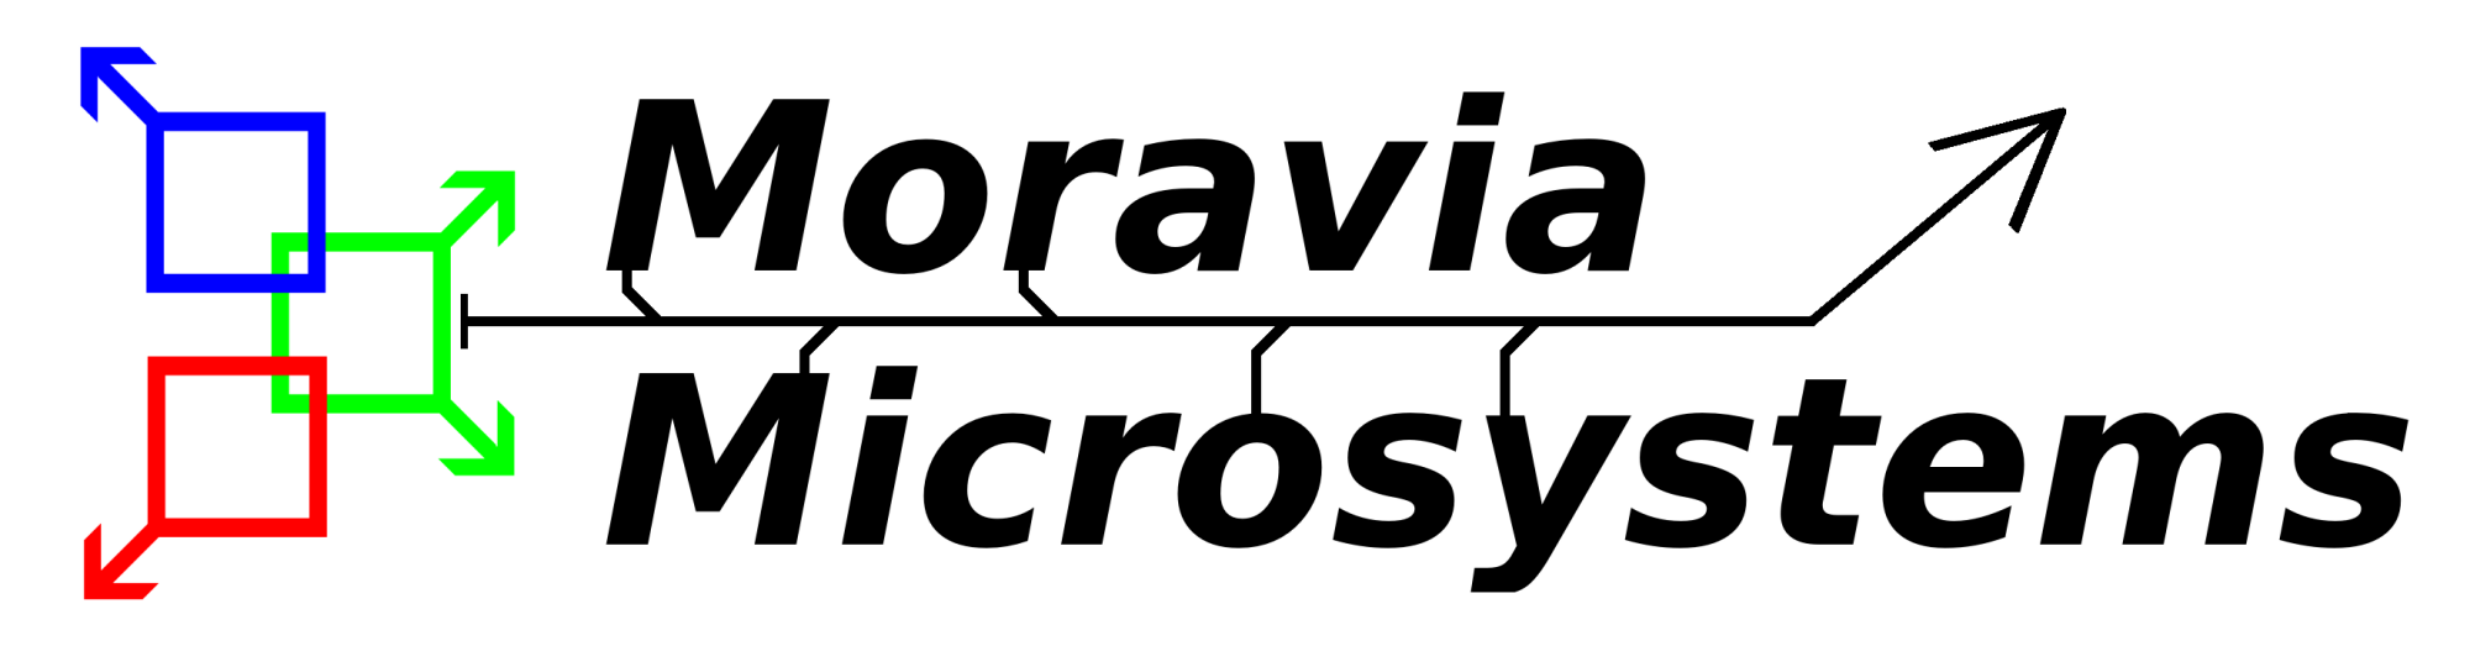
\includegraphics[width=.9\textwidth]{images/Moravia_Microsystems.png}
        \caption{\textit{Suggested logo of the company.}}
    \end{figure}
    \begin{center}
        \fontsize{35.83pt}{60pt} \selectfont{}
        \textbf{Business plan}
        \\[2cm]
        \fontsize{25pt}{30pt} \selectfont{}
        Comprehensive development tools\\
        for computerized hardware.
        \\[1cm]
        \fontsize{14.4pt}{20pt} \selectfont{}
        \textit{Martin Ošmera, Erik Chalupa, and Martin Madron \\ Brno, 2012}
    \end{center}
\end{titlepage}

\tableofcontents

\chapter{Preface}
    \section{Prologue}
        \begin{wrapfigure}{r}{120pt}
            \centering{}
            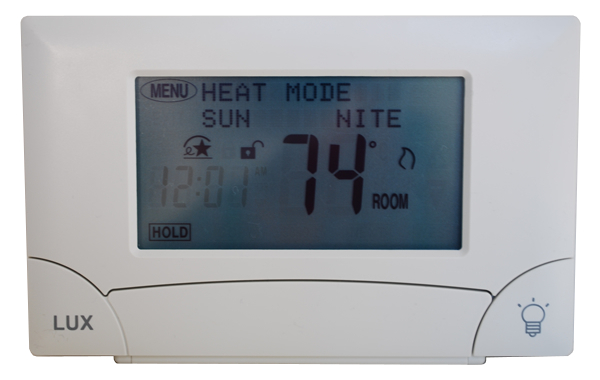
\includegraphics[width=110pt]{images/Lux_Products_Touch_Screen_Thermostat.jpg}
            \caption{A touch screen thermostat - an example of a device containing microcontrollers.}
        \end{wrapfigure}
        Look around you, computers and networks are everywhere, enabling an intricate web of complex human activities: education, commerce, entertainment, research, manufacturing, health management, human communication, even war. Of the two main technological underpinnings of this amazing proliferation, one is obvious: the breathtaking pace with which advances in microelectronics and chip design have been bringing us faster and faster hardware.

        Microcontrollers are one of the most interesting electronic devices of all, basically they are small computers integrated on a single chip, along with their memory, and other circuits, all of it packed into a single electronic device. These little computers are used in automatically controlled products and devices, such as automobile engine control systems, implantable medical devices, remote controls, office machines, appliances, power tools, toys and other embedded systems. By reducing the size and cost compared to a design that uses a separate microprocessor, memory, and input/output devices, microcontrollers make it economical to digitally control even more devices and processes. Mixed signal microcontrollers are common, integrating analog components needed to control non-digital electronic systems.

        \begin{wrapfigure}{l}{60pt}
            \centering{}
            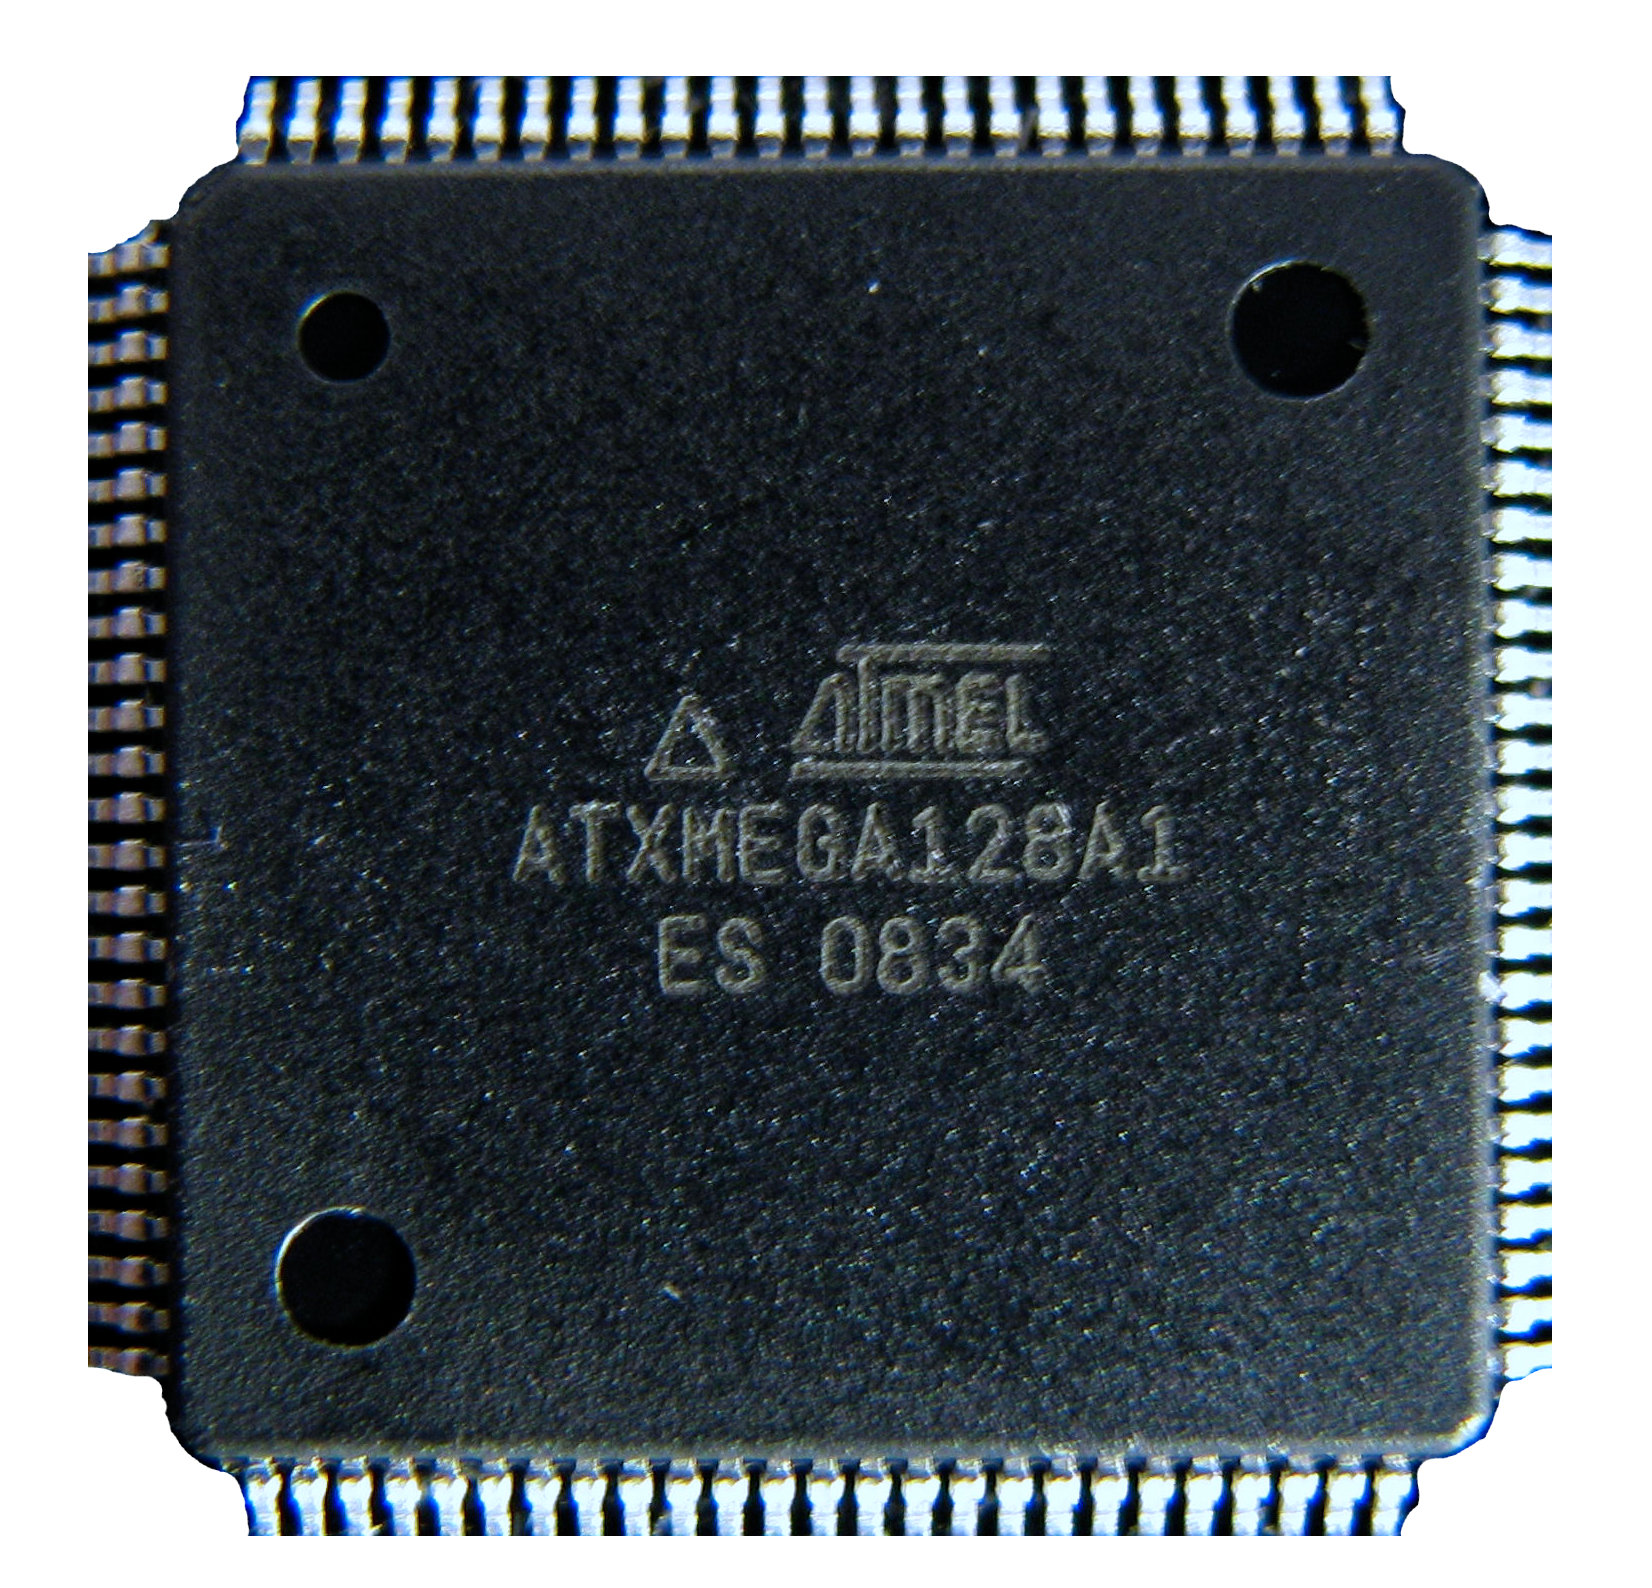
\includegraphics[width=50pt]{images/AVR_ATXMEGA_128A1.jpeg}
            \caption{AVR ATXMEGA microcontroller}
        \end{wrapfigure}
        However, there is a catch, programming these microcontrollers is a bit tricky, typically it requires a special equipment, i.e. specialized development tools, these tools are both hardware and software. Generally, the more sophisticated the development tools are, the more sophisticated the final product might become. It's practically impossible to successfully write a computer program without testing and debugging it, especially program for a microcontroller. In contrast to more complex computers, like personal computers, smart phones, etc., microcontrollers have significantly limited native debugging capabilities. And that's where complex simulation software, various development related hardware, and other tools like that, comes into the game. Most of these tools which currently available on the market, or as various freeware or open-source tools, have a great potential for improvement, not to mention that a great portion of these tools are merely a nice toys rather that complete and stable products.

        \begin{figure}[h!]
            \centering{}
            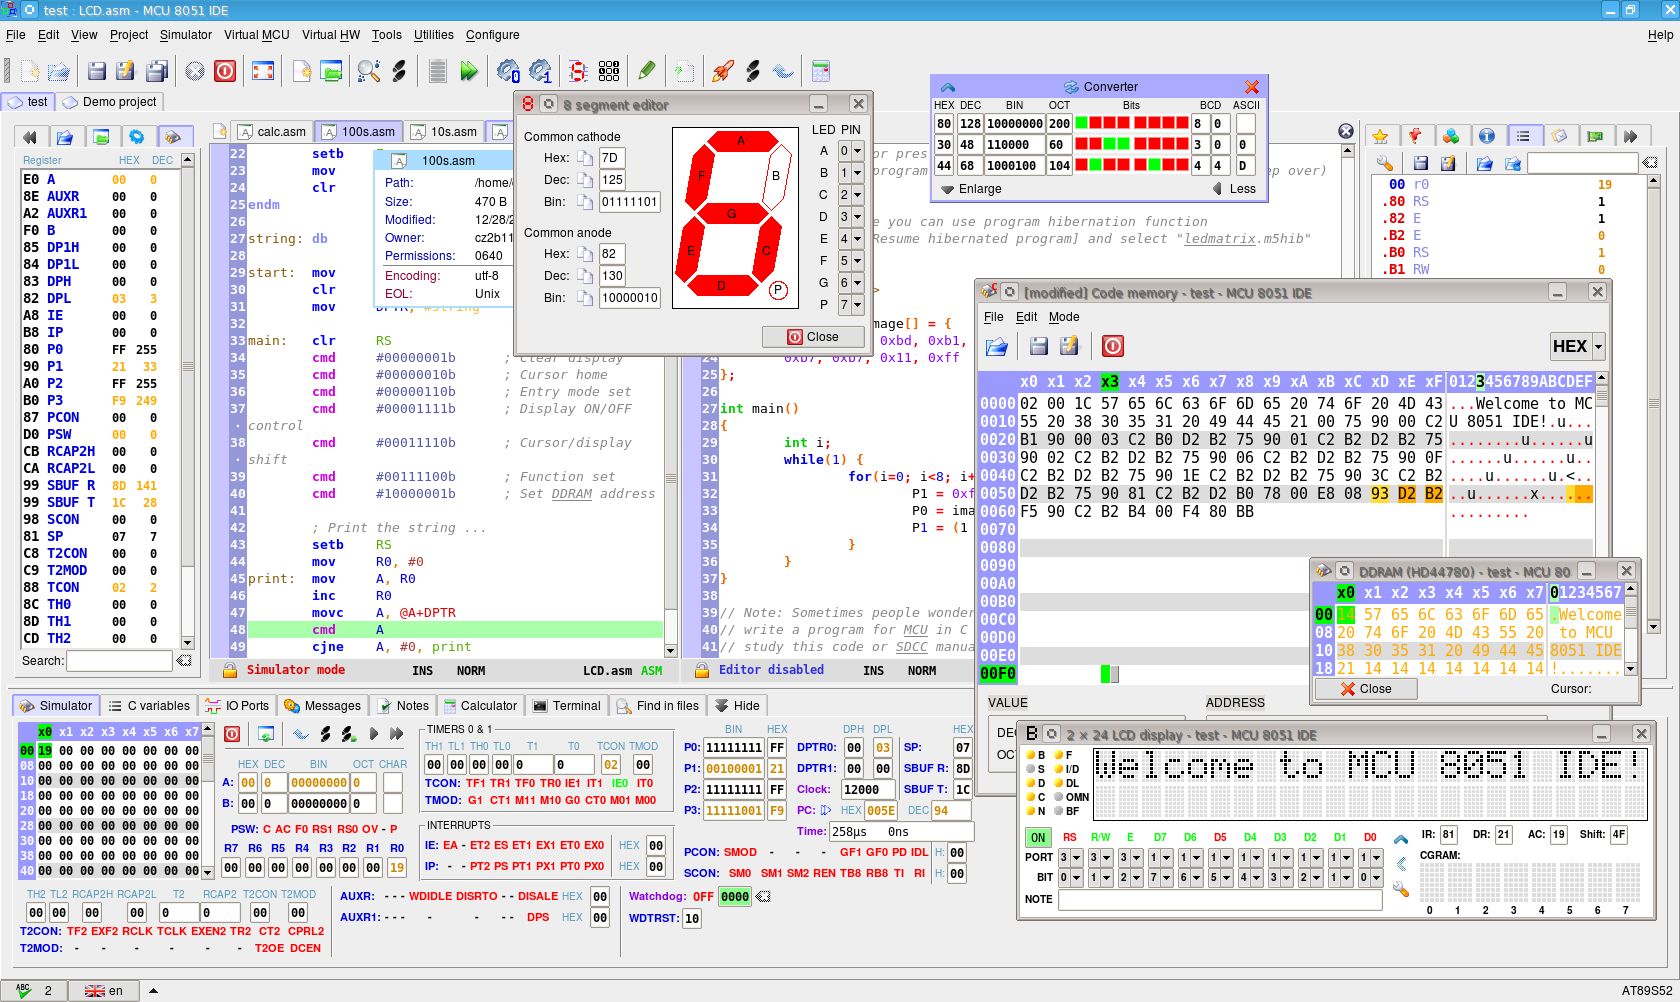
\includegraphics[width=.9\textwidth]{images/mcu8051ide_0.png}
            \caption{\textit{The \textbf{MCU~8051~IDE} project: A complete integrated development environment for 8051 based microcontrollers, available for Microsoft\textregistered{}~Windows\textregistered{} and GNU/Linux\textregistered{} written by one of the founders of the company - Martin Ošmera. The IDE currently used by a number of universities, other education institutions, and other subjects \textbf{around the globe}.}}
        \end{figure}

    \section{Vision of the project}
        The ultimate goal is to create an entirely new multiplatform development environment for microcontrollers and related hardware, using the most advanced technologies currently available. \textbf{Unlike other development tools} on the market, the result of this project is supposed to be highly modular and extensible, allowing us to distribute (sell) individual components for different purposes, and for different prices. In other words, there will be some ``main IDE'' (software), various hardware tools, and a set of additional plug-ins for the main IDE like:
        \begin{dinglist}{73}
            \item Package implementing \textbf{nodal analysis}, \textbf{transient analysis} and other methods for computer aided analysis and design of electronic circuits.
            \item Package for Unified Modeling Language (UML) (notable feature of this package might be \textbf{code generation from state charts})
            \item Package for LCD displays (simulators of character and graphical displays, font generators, etc.).
            \item Simulator extension package, code editor extension package, etc.
            \item Packages for digital potentiometers, thermometers, etc.
            \item Package for working with various communication protocols and interfaces.
            \item Package for working with embedded operating systems (we would either buy, or write our operating systems for individual microcontroller architectures).
            \item Package for development with \textbf{hardware definition languages} (VHDL, Verilog, etc.)
            \item Scientific package (visual programming, working with various diagrams, abstract machines, etc.)
            \item ... and other packages, depending on market demands ... also we would be potentially willing to write packages on demand to fit specific needs of particular customer.
        \end{dinglist}

        \begin{wrapfigure}{l}{150pt}
            \centering{}
            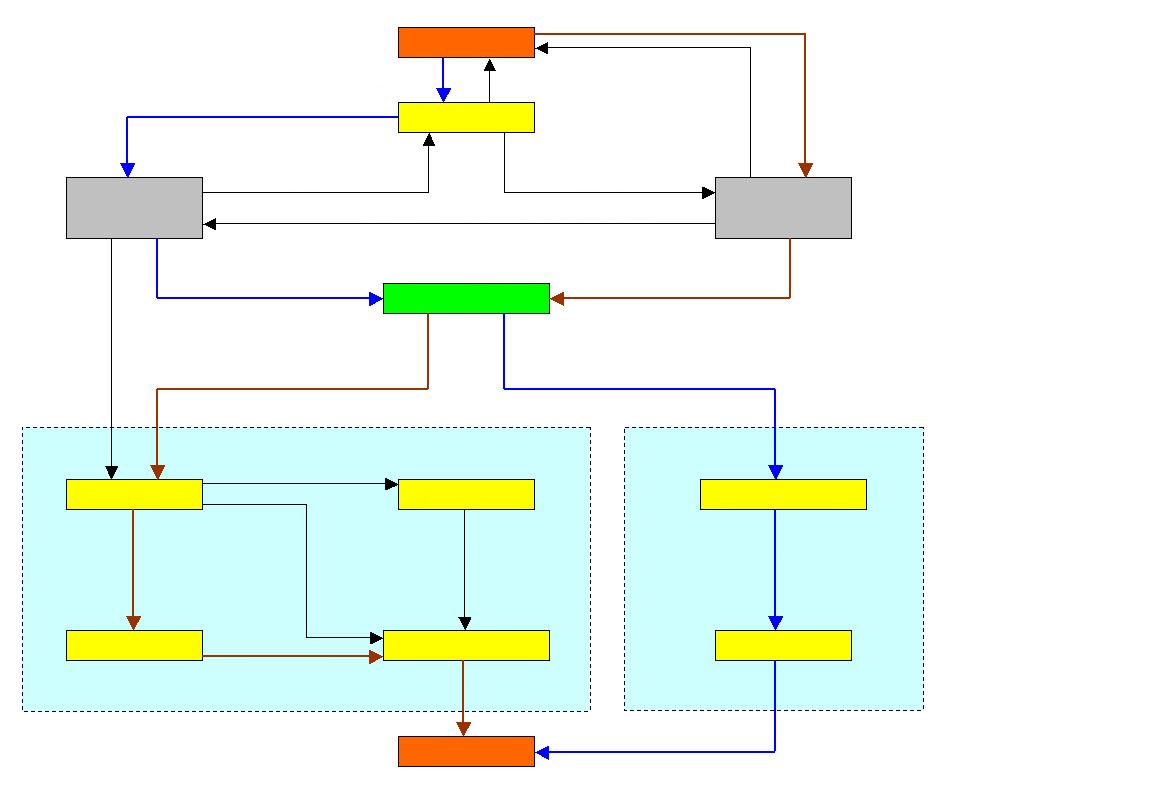
\includegraphics[width=140pt]{images/a_diagram.png}
        \end{wrapfigure}

        \textbf{The bottom line is} that the IDE would be entirely like a ``jigsaw'', this is one of the most important things which should make our products different from the others. The project counts on that we might profit more from the individual extension packages than from the main IDE itself. It likely that having only the main IDE would make us facing too heavy competition, but having a diverse portfolio of basically different but related products might prove to pose potential for rapid expansion of our efforts to different areas of technologies, and make our customers more willing to become dependent on our products. We believe that one the crucial rules of survival in this industry is to make others dependent on us, nobody wants to be dependent on a one big product so our strategy will be \textbf{divide~\& conquer}. There is also emerging potential in programs for GNU/Linux operating system, and since there are practically no development tools for microcontrollers currently available for this platform, we are going to be practically \textbf{the first ones to provide them}. This might also prove beneficial for our business.

    \section{The mission}
        \begin{quote}
            \textit{``It's better to reign in hell than to serve in heaven.'' -- John Milton}
        \end{quote}

        Our mission is clear, the company must make money, and make as much money as possible. In order to achieve that we have to be able to sell as many products as possible, and sell them for as high price as possible. We will do that by the following means:
        \begin{dinglist}{73}
            \item promoting our products everywhere possible (and reasonable),
            \item making it appear that we are bigger and more stable company than we really are,
            \item attempting to convince others that being dependent on us is for their good,
            \item providing high quality products,
            \item expanding to new territories and seek out new opportunities for business, and of course new products.
            \item take our work as a sort of art.
        \end{dinglist}

        \subsection{Potential customers}
            The highest number of our potential customers are most probably in India, USA, Germany, and Japan. The local Czech market is negligible, it's far too small to be promising, however, we expect to find some of our first customers among the Czech universities. Our customers expect reliable and advanced software and hardware solutions, proper equipment can considerably lower their running cost by saving valuable time. At the same time, the equipment should be easy to use as much as possible, however, these complex tools always require highly educated personal to handle them. Also we expect that they are willing to invest their money into tools like these even when they are not cheap because the money they invest will not go in vain.
            Our potential customers are:
            \begin{dinglist}{73}
                \item firms focused on development related to microcontrollers (like Honeywell, Alstom, etc. and a number of smaller companies),
                \item higher education institutions (the tools might be well used for education purposes),
                \item students and hobbyists, for these people the main IDE might be for free but only the main IDE, nothing more, or might consider some discounts or light versions.
            \end{dinglist}

        \subsection{The idea of innovation}
            \begin{dingautolist}{172}
                \item Advanced simulation capabilities including simulation of devices peripheral to the microcontroller, i.e. \textbf{nodal analysis}, etc.
                \item Multiplatform development tools allowing thousands, or tens of thousands, of engineers, scientist, and students, all around the world to use this kind of software and hardware tools also on GNU/Linux and Mac~OS~X operating systems.
                \item \href{http://en.wikipedia.org/wiki/Unified_Modeling_Language}{UML} (\textit{Unified Modeling Language}) tools for microcontrollers, the most notable one is automated generation of finite state machines (FSM) for microcontrollers. This probably poses a valuable potential in the field on industrial automation.
                \item Extensibility, we will be continuously writing additional plug-ins for the IDE.
                \item High simulation speed on host machines capable of multiprocessing.
                \item The project is supposed to bring some of the tools common to more a complex computers also to the world of microcontrolles, like \textbf{code profilers}, measurement of \textbf{software metrics}, \textbf{static code analysis}, real-time operating systems, etc., some of these are already available on the market but our solutions are supposed to be more complex and advanced.
            \end{dingautolist}

        \subsection{Potential future}
            Open-source software probably will be the most valuable ally for us, but it time it might also endanger our business, in time tools like this might become open-source, effectively inhibiting many of business activities like the one we intend to conduct. We should be prepared for this in advance, so in case the IDE and its associated tools become successful, we will have seriously consider expanding to other areas, like:
            \begin{dinglist}{73}
                \item various versatile devices for industrial automation,
                \item field-programmable gate arrays (\href{http://en.wikipedia.org/wiki/Programmable_gate_array}{FPGA}),
                \item our own microcontrollers and/or microprocessors (this might be too ambitious),
                \item other kinds of software (genetic programming, neural networks, etc.),
                \item in case of a big success of the company, we could found and/or buy a few subsidiaries to form a concern with us,
                \item et catera.
            \end{dinglist}

        \subsection{Intellectual property}
            The software is supposed to be proprietary, probably licensed under EULA license or something very similar, the hardware as well. We do not intend to issue software patents nor any other kind of patents.

\chapter{Detailed description of the planned products}
    \begin{quote}
        \textit{``If you are going to steal software, steal it from us.'' -- Jeff Raikes (Microsoft executive)}
    \end{quote}

    \section{Software}
        Our main product will be software. Currently there are plenty of software products focused on a development which is directly related to microcontrollers, there already are companies developing similar software and hardware as we intent to do, even independent individuals are doing so. However, there is still an area which is not entirely covered by these products, and that's where we should focus our efforts. So besides the main products, we are also about to experiment in certain uncharted areas of the market.

        \begin{figure}[h!]
            \centering{}
            
\includegraphics[width=.5\textwidth]{images/os.png}
            \caption{Our target platforms.}
        \end{figure}

        \subsection{Concrete products}
            \begin{dinglist}{73}
                \item Multitarget Development System (MDS), The Main IDE: basic product but not the main source of our financial profit, suggested price: ca. \$170 a license for standard version (including electronic circuit simulation), and ca. \$99 for light version (without electronic circuit simulation).
                \item Package for circuit simulation (something like PSpice, Electronics Workbench, Tina, etc.) suggested price: ca. \$99 a license.
                \item UML extension package: main feature would be automated code generation from UML state charts, etc., this particular product might significantly ease development of applications involving finite state automata, etc. suggested price: ca. \$500 a license.
                \item Scientific extension package, enabling usage of many basically ``useless nonsenses'' like the visual programming and other highly impractical things, suggested price: \$300 a license.
                \item Various additional simulators, like simulator of \href{http://en.wikipedia.org/wiki/Hitachi_HD44780_LCD_controller}{HD44780} driven LCD display (and graphical displays, of course), and similar tools, suggested prices for individual packages: from \$10 to \$1,000 a license.
                \item Packages for working with various communication protocols, like USB, etc., suggested prices for individual packages: from ca. \$50 (simple protocols like: SPI, UART, USART, $I^2C$, etc.) to ca. \$250 (sophisticated protocols like: CAN, USB, Ethernet, IP, etc.) a license.
                \item Packages for working with embedded operating systems, mostly our own operating systems, suggested prices for individual packages, including the operating systems: from \$100 to \$1,000 a license.
                \item Extension packages written, on customer demand, to fit individual needs of particular customers, prices for these packages would be thousands, or tens of thousands, dollars.
                \item In time, we would come with other products.
            \end{dinglist}

        \subsection{What we will not do}
            \begin{dinglist}{73}
                \item We will not write our own C and/or C++ compiler(s). There are GCC and SDCC compilers freely available on the Internet as open-source projects, their licenses allows us to use them for our activities. We could save a big portion of valuable time by using them, and there is no point in reinventing the wheel. Although if we find this to be a potentially good investment, we might implement it.
                \item Stick to the main IDE (Multitarget Development System). There other IDEs available, and even if ours would be the best one ever, it probably still wouldn't be good enough to maintain the company indefinitely. And we wouldn't withstand the competition forever anyway.
                \item Make our software open-source, and hardware open-core, it would make it too easy to steal; and for the majority of end-users, it would be no advantage anyway.
                \item Become dependent on particular operating system, like Microsoft Windows or MAC OS X.
                \item Make our software unavailable to all people who won't buy it anyway, like students, it's only good for us when there is a plenty of people using it, even when we don't get money from all of them.
            \end{dinglist}

        \subsection{What might make us better than the others}
            \begin{dinglist}{73}
                \item There are no professional grade IDEs capable of simulation of certain important peripherals, like LCD displays, various controllers, etc. Reliable and well written set of individual simulators for these devices could significantly ease the development process and thus make our products more attractive. These additional simulators would be sold as individual packages allowing customer to configure the IDE to fit his or her specific needs.
                \item Most of the MCU simulators currently available are too slow because they are mostly products of developers who focus primarily on something else.
                \item There are almost no professional grade IDEs capable to run on other operating system than Microsoft\textregistered{}~Windows\textregistered{} but our products would run on Microsoft Windows, GNU/Linux, and Mac OS X, so there is a good chance that we could quickly cover this slowly emerging portion of the market.
                \item Most of the development tools currently available are clumsy, there are not well written, slow, instable, etc. That's caused by the fact that the people writing them lack the necessary experience and expertise. We can easily profit from years of experience gained from the MCU~8051~IDE project, a successful worldwide spread open source IDE for MCS-51 based devices.\footnote{The MCU~8051~IDE is today commonly used at universities and similar institutions all around the world, it's a project which in certain aspects can match commercial products of similar kind developed by entire companies. The experience from this project might be very beneficial. We can provide such products in considerably less time and with considerably higher quality than our competitors.}
                \item People who write development tools for microcontrollers usually doesn't have a background in the kind of software development that we do, they can write software, more or less, but they are not good programmers. We could also gain advantage from software technologies like \href{http://en.wikipedia.org/wiki/Qt_framework}{Qt framework}, \href{http://en.wikipedia.org/wiki/Small_Device_C_Compiler}{SDCC compiler}, \href{http://en.wikipedia.org/wiki/GNU_Compiler_Collection}{GCC compiler}, GNU/Linux operating system, etc., these things are usually unknown to writers of similar products, and even when they are aware of them, they are not able to use them.
            \end{dinglist}

        \subsection{Random remarks to the software}
            \begin{dinglist}{73}
                \item the main IDE:
                    \begin{dinglist}{75}
                        \item There will be basically three separate parts running as separate processes, one for the GUI, one for compiler (SDCC or GCC), and one the simulator engine. We can take \textbf{very interesting advantages} of decoupling the GUI and the simulator engine as separate processes, one is performance on multi-core CPU machines, one is ability to run simulator on a different machine than the GUI, and the most important one is stability. Simulator engine is a component which would be a subject to extensive automated testing, it's not too hard to prepare a set of test cases for an automated testing environment which will do the work for us, however, it's hard to test the GUI automatically, so naturally most of bugs in the software will be in the GUI. When the GUI crash, the simulator will stop but remain functional, and mostly unaffected by the crash of the GUI, allowing for the entire application to cope with the crash more easily.
                        \item Everything possible will be written to be general in respect to the target microcontroller architecture, and configurable by user.
                        \item Files generated and/or used by the IDE, like project definition file, various configuration, etc., files, will be human readable or at least not binary, except for cases for which there is not other way. Asset of this feature is that user will be able to mess with those files, e.g. generated and/or process them by his or her own scripts and other tools.
                        \item Everything in GUI must look modern, the GUI should be full of tiny little gadgets in order to make it appear that it's \textbf{not an ordinary software}, it's the Software.
                        \item The first version(s) released will probably be useful only as education software, since many of features crucial for a real development might be missing there.
                    \end{dinglist}
                \item Individual extension packages:
                    \begin{dinglist}{75}
                        \item Some of them will extend GUI of the main IDE, some of the will extend simulator, in both cases they should be \textbf{decoupled as possible}. They should communicate with the GUI via interprocess communication, not integrated directly into the main app. Extensions for the simulator engine, like simulators of displays, etc., should consist of two pars: GUI and the internal logic. The internal logic should integrate directly into the simulator engine, for performance reasons, and the GUI should run in a separate process, also for performance reasons and also to ensure higher stability of the software.
                        \item People usually don't like big, complex, and expensive things, rather they prefer a set of small, easy to understand, and inexpensive fractions of something bigger, even when that's merely an illusion. So let's provide it that way, the main advantage of this approach, from our point of view, is that we can sell them something big, complex, and very expensive part by part. Suppose I want an IDE for microcontrollers, ok, I buy it and let's say I am satisfied, for now, but later I might realize that I want also this tiny little piece of additional software, ok, I buy it and let's say I am satisfied, but later ...
                    \end{dinglist}
                \item Installation process:
                    \begin{dinglist}{75}
                        \item for Windows we might use one of the following installers:
                            \begin{dinglist}{72}
                                \item \href{http://nsis.sourceforge.net/Main_Page}{NSIS} (Nullsoft Scriptable Install System) -- an open source system to create Windows installers,\footnote{This add-on might also be useful: \url{http://www.graphical-installer.com/joomla/}.}
                                \item \href{http://www.jrsoftware.org/isinfo.php}{Inno Setup} -- a free installer for Windows programs,
                                \item \href{http://www.flexerasoftware.com/products/installshield.htm}{InstallShield} -- a proprietary system to create Windows installers,
                            \end{dinglist}
                        \item for Linux we use rpm-build (for RPM packages) and dpkg-deb (for DEB packages)
                    \end{dinglist}
            \end{dinglist}

    \clearpage
    \section{Hardware}
        When writing code for an application, it is advantageous to have development hardware which can ease and speed up the work. This hardware can create conditions similar to the target application and developer can develop and debug the application in the comfort of his or her office. Hardware, however, might require a considerable financial investment, but the asset can be much shorter "time to market" product. Development hardware also plays and essential role in bringing the code into the real world where all stimuli and influences that simulator might not have taken into account are revealed.
        \begin{figure}[h!]
            \centering{}
            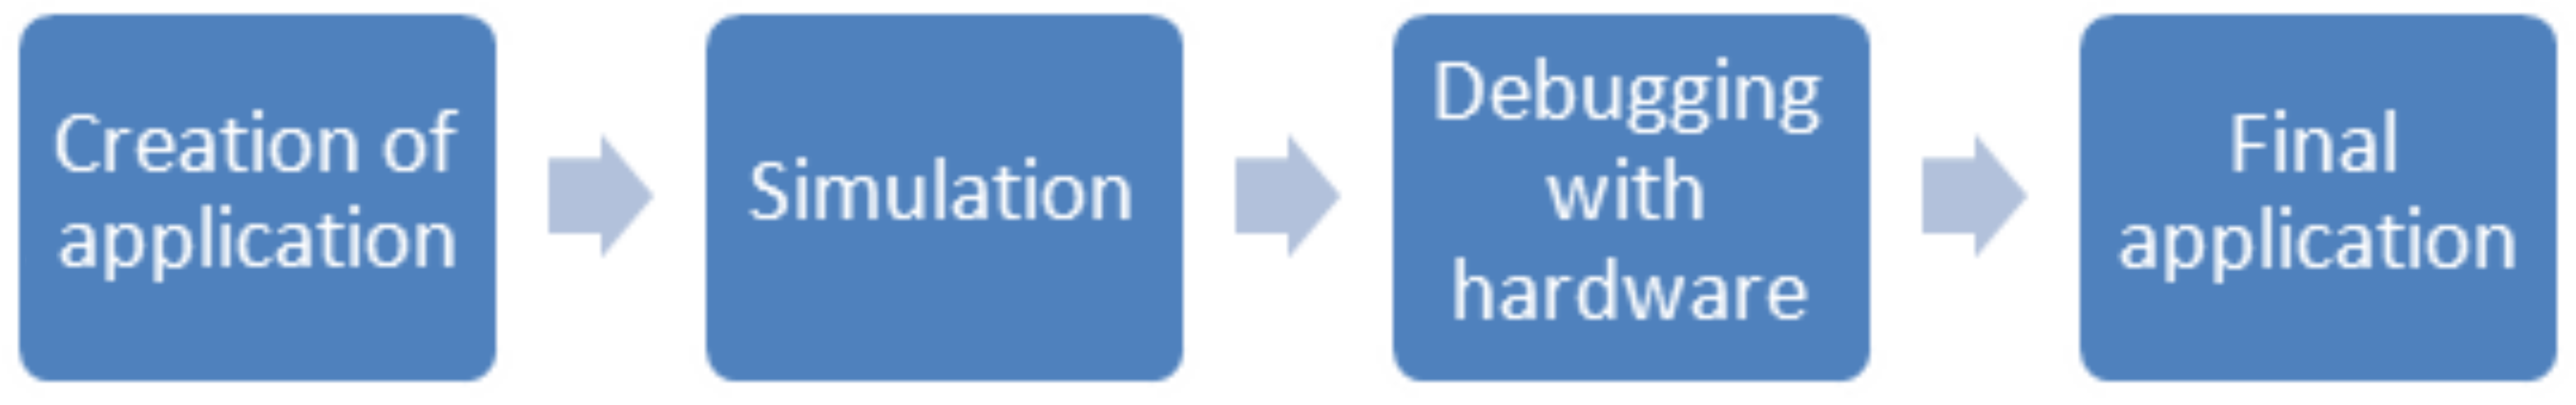
\includegraphics[width=.9\textwidth]{images/prvni_obr_pod_hardware.png}
            \caption{Role of development hardware in the process of product development.}
        \end{figure}

        There are several kinds of development hardware which can be used with our products, their basic types are described below (mentioned costs and prices are without taxes).
        \begin{figure}[h!]
            \centering{}
            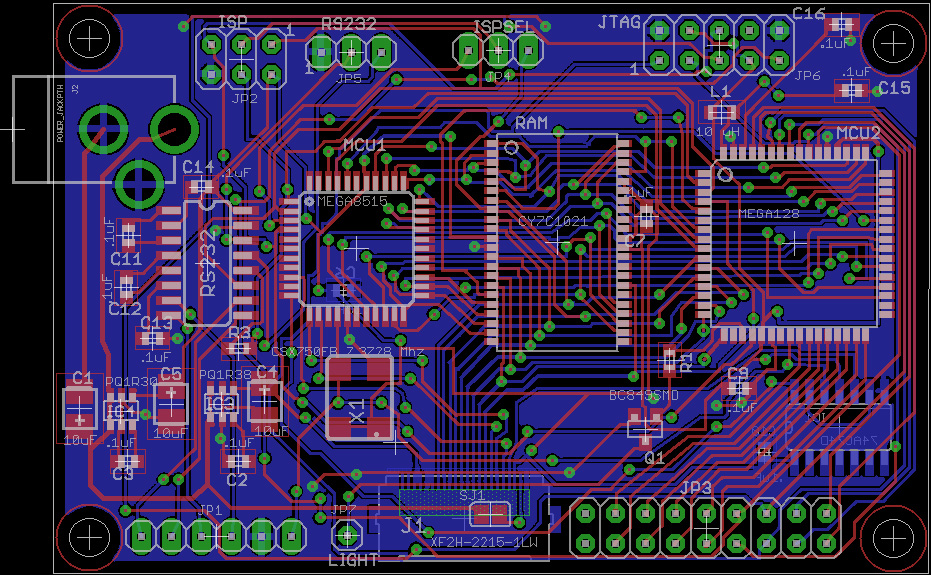
\includegraphics[width=.7\textwidth]{images/pcb.png}
            \caption{A printed circuit board digram \textit{(AVCX Graphics LCD Controller)}.}
        \end{figure}

        \subsection{MCU programmers}
            This equipment is needed for loading code into the microcontroller; in our case, it is only one microcontroller on the printed circuit board (besides MCU interfacing with the host computer, probably via the Universal Serial Bus).
            \begin{figure}[h!]
                \centering{}
                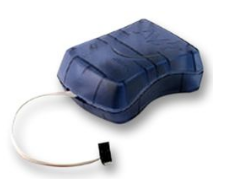
\includegraphics[width=.2\textwidth]{images/programmer.png}
                \caption{An MCU programmer manufactured by a competitor company.}
            \end{figure}

            \begin{table}[h!]
                \begin{tabular}{lr}
                    microcontroller         & 80~CZK        \\
                    connectors              & 50~CZK        \\
                    printed circuit board   & 50~CZK        \\
                    other parts             & 50~CZK        \\\hline
                    total                   & 230~CZK
                \end{tabular}
                \caption{Estimated production cost for a piece}
            \end{table}

            \subsubsection{Estimated selling price}
                Basically the most important factor determining the selling price is the number of microcontrollers supported by the programmer. In the beginning our programmers will support only the basic series of microcontrollers currently available on the market. In the future, however, we are intent to create programmers supporting nearly all available series. We also plan to create a universal programmer supporting more families of microcontrollers (e.g. PIC, AVR, 8051, etc.) at once. We are able to offer first versions of our programmers for approximately 500~CZK. Like with many other products, manufacturing of these electronic devices might become substantially cheaper when dealing with large quantities, according to our estimations we make make up to 40\% discount on all parts by buying then in larger quantities at once.

        \subsection{In-Circuit Debuggers (ICD)}
            Basically they are just advanced programmers, they are able to program the microcontroller and also step through the running program directly in the hardware.

            \begin{figure}[h!]
                \centering{}
                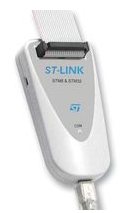
\includegraphics[width=.15\textwidth]{images/debuger.png}
                \caption{A ICD manufactured by a competitor company.}
            \end{figure}

            \begin{table}[h!]
                \begin{tabular}{lr}
                    microcontroller         & 100~CZK       \\
                    connectors              & 100~CZK       \\
                    printed circuit board   & 100~CZK       \\
                    auxiliary circuits      & 100~CZK       \\
                    other parts             & 80~CZK        \\\hline
                    total                   & 480~CZK
                \end{tabular}
                \caption{Estimated production cost for our first version}
            \end{table}

            \subsubsection{Estimated selling price}
                Selling price of the first version of the ICD will be approximately 1200~CZK. However, the price might drastically increase as the number of supported microcontrollers grows. The prices of ICDs varies in the range of tens thousand CZK.

        \subsection{Evaluation boards}
            This kind of hardware tool integrates some of the most common types of hardware peripherals on one printed circuit board (PCB). The advantage of these tools is that before uploading a program into the application the user can test overall functionality and perform certain level of debugging, also these devices are heavily used for educational purposes. But production costs of these tools are usually a lot bigger than for programmers and in-circuit debuggers. Evaluation boards often include an MCU programmer as their integral part.

            \begin{figure}[h!]
                \centering{}
                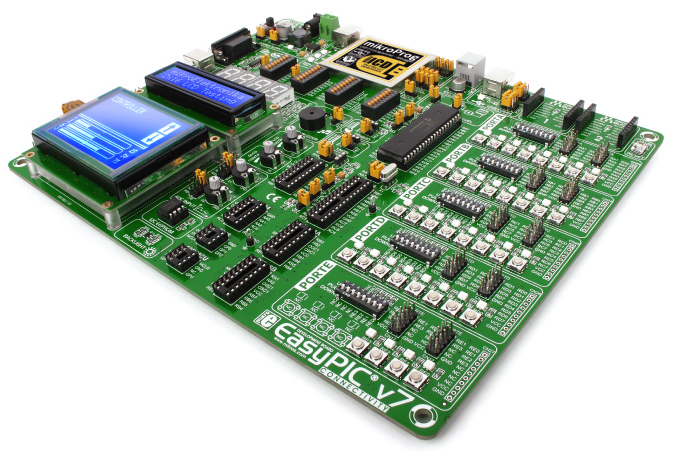
\includegraphics[width=.5\textwidth]{images/snapshot0.png}
                \caption{An evaluation boards made by the \href{http://www.mikroe.com/}{MikroElektronika company} (probably out main potential competitor).}
            \end{figure}

            \subsubsection{Estimated production cost}
                Cost of production of these boards varies with their complexity. When starting the business will have more than version at in our portfolio with highly variating complexity level. The following estimate was made for a board fully comparable to the depicted board made by the MikroElektronika company.
                \begin{table}[h!]
                    \begin{tabular}{lr}
                        microcontrollers        & 120~CZK       \\
                        connectors              & 430~CZK       \\
                        printed circuit board   & 250~CZK       \\
                        LCD display             & 250~CZK       \\
                        auxiliary circuits      & 80~CZK        \\
                        other parts             & 270~CZK       \\\hline
                        total                   & 1400~CZK
                    \end{tabular}
                \caption{Estimated production cost for one a more complex piece.}
                \end{table}

            \subsubsection{Estimated selling price}
                The selling price varies in dependence on complexity and size of the board. The mentioned board should be sold for about 2200 - 2600 CZK.

        \subsection{Other tools}
            \begin{quote}
                \textit{``Good artists copy, great artists steal.'' -- Pablo Picasso}
            \end{quote}
            Other tools might include:
            \begin{dinglist}{73}
                \setlength{\itemsep}{-3pt}
                \item various accessories for our other tools (e.g. displays, keypads, etc.),
                \item bridges (e.g. USB->UART),
                \item various analyzers,
                \item cables, etc.
            \end{dinglist}

    \section{Services}
        \subsection{Technical support}
            We intent to provide ``high quality technical support'' for our products, like Microsoft does. Beside this ``high quality technical support'', there should be discussion forum on our web pages, and it should be also possible to contact the developers using email or phone.

        \subsection{Advertisement}
            Out commercials are supposed to be distributed using the Internet, that means: our web pages, YouTube, FaceBook, Twitter, Wikipedia, etc. The images and motion pictures should be playful, and should make us look like a creative team of software developers, nice music, and nice visual effects. However, inadequate and/or misunderstood advertisement might put our efforts in jeopardy despite even flawless solution of our products. A good example of a well made advertisement might be this: \url{http://www.home.agilent.com/agilent/product.jspx?cc=CZ&lc=eng&ckey=1297113&nid=-34346.0.00&id=1297113}

    \section{Production process}
        \enlargethispage{4\baselineskip}
        \begin{wrapfigure}{r}{120pt}
            \centering{}
            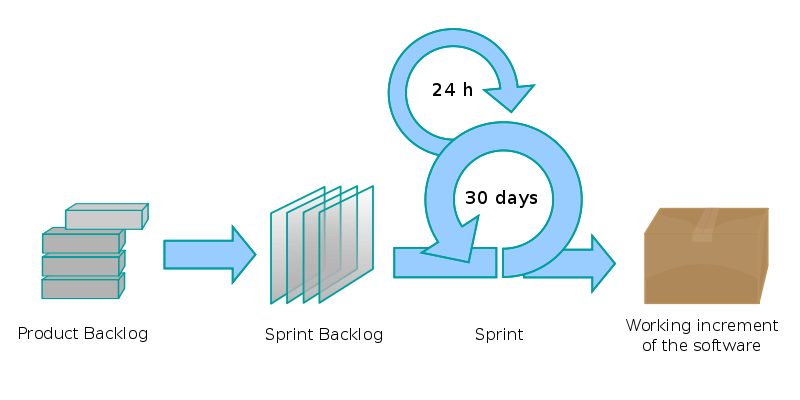
\includegraphics[width=110pt]{images/Scrum_process.png}
            \caption{Scrum, an incremental framework for project management.}
        \end{wrapfigure}
        Small teams are usually best organized when they are self organized. So we suggest application of an agile software development process, the best choice might be the Scrum, although other methodologies are also applicable, e.g. the Waterfall model.
        Suggested scenario:
        \begin{dinglist}{73}
            \item there are a few teams focusing on different, but related, products and/or their components,
            \item each team start as one-man team,
            \item work is planned for short periods of time, at the end of this period the team presents the result to the ``product owner'' (it would be either a commission or some dedicated person),
            \item everything is planned, however, the plan is highly adaptive in order to make the teams operative,
            \item unless explicitly specified otherwise, everything is confidential (contracts might insist on that, if necessary).
        \end{dinglist}

\chapter{Analysis}
    \section{The market}
        \subsection{Suppliers}
            We need suppliers in the following fields:
                \begin{dinglist}{73}
                    \item web pages (domains: www.moravia-microsystems.com, www.moraviamicrosystems.com, www.moravia-microsystems.cz, www.moraviamicrosystems.cz)
                    \item advertisement
                    \item printed circuit boards, we might choose from companies like these:
                    \begin{dinglist}{75}
                        \item \href{http://www.apama.cz/}{APAMA SYSTEM}: Czech manufacturer with good prices,
                        \item \href{http://www.semach.cz/}{SEMACH}: oriented mainly on development and prototypes (Singlesided: 38~CZK/dm$^2$, Doublesided: 58~CZK/dm$^2$; Trough Hole Doublesided: 148~CZK/dm$^2$),
                        \item \href{http://www.a3.cz}{A3}: also PCD supplier from Taiwan and China,
                        \item \href{http://www.tistaky.cz/}{Tistaky}: Czech manufacturer.
                    \end{dinglist}
                \end{dinglist}

        \subsection{Competitors}
            Our main competitor will be the \href{http://www.mikroe.com/}{MikroElektronika company} (~Serbia, Europe), they do basically the same thing what we intent to do, however, our products are supposed to be far superior. What these people do is merely scratching the surface, we indent do go far beyond this basic level. Another interesting company is the \href{http://www.keil.com/}{KEIL company} (Europe,~Germany), they seem to be pretty good but they are targeting on different MCU architectures. In time, we might have to compete with them as well, and win, if possible. Other companies, like UNIS, etc. pose no threat for us, they focus on different fields of the market and probably lacking a real potential to compete with us.
            \begin{table}[h!]
                \centering{}
                \begin{tabular}{cp{40pt}c}
                    
\includegraphics[width=120pt]{images/MikroElektronika_logo.png}
                        & ~ &
                    
\includegraphics[width=60pt]{images/KeilARM.jpg} \\
                \end{tabular}
            \end{table}

        \subsubsection{MikroElektronika}
            MikroElektronika produce entire development toolchains for all major microcontroller arhitectures. They make development boards, compilers, accessory boards, additional software and books for microcontrollers. They offer:
            \begin{dinglist}{73}
                \item PIC Development Boards
                \item PIC Compilers
                \item dsPIC Development Boards
                \item PIC24 and dsPIC33 Tools, Programmer
                \item dsPIC30/33 and PIC24 Compilers
                \item PIC32 Development Boards
                \item PIC32 Compilers
                \item AVR Compilers
                \item AVR Development Boards
                \item ARM Compilers
                \item ARM Development Boards
                \item 8051 Compilers
                \item 8051 Development Boards
            \end{dinglist}

            So how do we beat MikroElektronika, at the beginning we will do almost everything the same as they do but with the aforementioned innovations which we believe carry a valuable business potential. Also their software is mostly a bit immature which is weak spot which we could exploit. The company is based in eastern Europe in Serbia (former part Yugoslavia).

        \subsubsection{Keil}
            The Keil\texttrademark products from ARM include C/C++ compilers, debuggers, integrated environments, RTOS, simulation models, and evaluation boards for ARM, Cortex-M, Cortex-R, 8051, C166, and 251~processor families.

            What do they offer:
            The $\mu$Vision IDE from Keil combines project management, make facilities, source code editing, program debugging, and complete simulation in one environment. The $\mu$Vision editor and debugger are integrated in a single application that provides a seamless embedded project development environment.
            \begin{dinglist}{73}
                \item Keil's software:
                    \begin{dinglist}{75}
                        \item complete support for Cortex-M, Cortex-R4, ARM7, and ARM9 devices,
                        \item industry-leading ARM C/C++ Compilation Toolchain,
                        \item $\mu$Vision4 IDE, debugger, and simulation environment,
                        \item Keil RTX deterministic, small footprint real-time operating system (with source code),
                        \item TCP/IP Networking Suite offers multiple protocols and various applications,
                        \item USB Device and USB Host stacks are provided with standard driver classes,
                        \item complete GUI Library for embedded systems with graphical user interfaces,
                        \item ULINKpro enables on-the-fly analysis of running applications and records every executed,
                        \item Cortex-M instruction,
                        \item complete Code Coverage information about your program's execution,
                        \item execution Profiler and Performance Analyzer enable program optimization,
                        \item numerous example projects help you quickly become familiar with MDK-ARM's powerful, built-in features,
                        \item CMSIS Cortex Microcontoller Software Interface Standard compliant.
                        \item et catera ... (8051 Development Tools, C166 Development Tools, Evaluation Boards).
                    \end{dinglist}
                \item Keil's hardware:
                    \begin{dinglist}{75}
                        \item starting price is \$99 (basic environment for 8-bit MCUs, but they focus mainly on ARM microcontroller architecture),
                        \item MDK-ARM costs \$4895 (92~358 CZK)
                        \item MDK-ARM-B (basic) costs \$2895 (54~622 CZK)
                        \item MDK-ARM-T (term) costs \$1958 (36~943 CZK)
                        \item et catera ... (in short their hardware tools aren't cheap).
                    \end{dinglist}
            \end{dinglist}

            So how do we beat Keil, first we have to realize that they are Germans, and all Germans have one thing in common: they are much better paid we are (eastern European people) so we can easily be cheaper then them. Also we intent to bring a few new innovations which they just don't have, and it doesn't seem likely that they will acquire them in short time (like circuit simulation connected with MCU simulation, Windows/Linux/Mac IDE).

        \subsubsection{Others}
            Besides that there are plenty of other companies, we have picked up these two (Keil and MikroElektronika) just as examples, it exceeds purpose of this document to focus separately on every possible competitor in the world. Our products are still supposed to be unique and bring new valuable innovations into the market.

    \clearpage
    \section{SWOT analysis}
        \begin{table}[h!]
            \centering{}
            \begin{tabular}{|p{.5\textwidth}|p{.5\textwidth}|}
                \multicolumn{1}{>{\columncolor[rgb]{0.1,0.7,0.0}}c}{\color{white}{\textbf{Strengths}}}
                    & \multicolumn{1}{>{\columncolor[rgb]{0.90,0.7,0.0}}c}{\color{white}{\textbf{Weaknesses}}} \\

                % Strengths:
                \begin{dinglist}{249}
                    \setlength{\itemsep}{-3pt}
                    \item Simulation of MCU peripherals, i.e. circuit simulation.
                    \item Automated code generation from UML state charts.
                    \item Modular development framework.
                    \item Advantage of already written open-source C compilers.
                    \item High performance, stability, and security, by software design.
                    \item Fancy GUI of the Qt framework.
                    \item Multiplatformness of the software.
                    \item Target MCU architectures.
                    \item Low-cost workforce.
                    \item Experience from the MCU~8051~IDE project.
                    \item We might easily expand to more perspective areas of business from this starter product.
                \end{dinglist}  &

                % Weaknesses:
                \begin{dinglist}{74}
                    \setlength{\itemsep}{-3pt}
                    \item Inexperienced team.
                    \item We are in the Eastern Europe.
                    \item Probably there is no potential to create a cash cow.
                    \item The project might be too sophisticated.
                    \item We might not be able to deliver the final product with satisfactory quality.
                \end{dinglist}  \\

                \multicolumn{1}{>{\columncolor[rgb]{0.3,0.3,1.0}}c}{\color{white}{\textbf{Opportunities}}}
                    & \multicolumn{1}{>{\columncolor[rgb]{1.0,0.1,0.1}}c}{\color{white}{\textbf{Threats}}} \\

                % Opportunities:
                \begin{dinglist}{73}
                    \setlength{\itemsep}{-3pt}
                    \item Microcontrollers are heavily used in today's industry.
                    \item If we succeed, nobody will be able to match us.
                    \item We could expand to our own microcontrollers.
                \end{dinglist}  &

                % Threats:
                \begin{dinglist}{247}
                    \setlength{\itemsep}{-3pt}
                    \item Our products are supposed to be honestly beneficial and innovatory.
                    \item Companies like MikroElektronika, etc., might pose a hard competition for us.
                    \item There might not be enough customers to keep the company alive.
                    \item This product might be too specialized to be profitable enough.
                    \item There are similar products for free.
                    \item We might not gain satisfying credibility.
                \end{dinglist}  \\
                \hline
            \end{tabular}
            \caption{SWOT analysis}
        \end{table}

        \subsection{Analysis of the strengths}
            I am strongly convinced that the project has some very serious advantages, you must understand that is a really not an ordinary IDE. This is an entirely different way of approach.
             \begin{description}
                \item[Simulation of MCU peripherals:]
                    this feature is the cornerstone of this innovation, no other set development tools currently available on the market has this feature supported as we intent to. Various peripherals connected to the microcontroller are very important, usually the only thing the MCU has to do is to control these peripherals, so having the simulated by software might pose a valuable asset for our customers.
                \item[Automated code generation from UML state charts:]
                    this might significantly ease development process of applications \href{http://en.wikipedia.org/wiki/Finite-state_machine}{involving finite state automata}, and it it also poses the potential to make our customers more dependent on our products. Finite state automata (finite state machines) are heavily used in today's software industry, so having this supported the software might be very valuable.
                \item[Modular development framework:]
                    it is our believe that having the software divided into several separate packages, having each of them sold separately for different price, and thus allow our customers to choose exact configuration of their development environment to fir their particular needs. We are supposed to benefit from this by being able to make more money by selling individual extension packages than by selling the main IDE itself.
                \item[Advantage of already written C compilers:]
                    other companies developing tools like these often write their own compilers for the C language, \footnote{C language is an extremely popular technology in the field of MCU programming; while BASIC, Pascal, etc., are more merely a toys rather than serious industrial technologies.} we would skip this step and use the \href{http://en.wikipedia.org/wiki/Small_Device_C_Compiler}{SDCC} and the \href{http://en.wikipedia.org/wiki/GNU_Compiler_Collection}{GCC} compiler. These compilers are distributed and so called free software (free as in freedom), that practically means that they are open-source software. License used for these compilers is GNU~GPL, this allows us to use them as external programs, which our software will strongly depend on, without having to ask for permission from their copyright holders.\footnote{The \href{http://en.wikipedia.org/wiki/Free_Software_Foundation}{Free Software Foundation} (which holds the copyright of several notable GPL-licensed software products and of the license text itself) asserts that an executable which uses a dynamically linked library is indeed a derivative work. This does not however apply to separate programs communicating with one another.}\footnote{\href{http://www.gnu.org/licenses/gpl-faq.html\#NFUseGPLPlugins}{Basic questions about the GNU Project, the Free Software Foundation, and its licenses}}
                \item[High performance, stability, and security, by design:]
                    the software is supposed to work as a ``network'' of mutually connected processes, i.g. threads and separate processes communicating via out proprietary communication protocol over UDP/IP, or TCP/IP, or basically arbitrary mechanism of interprocess communication. This means that the software can easily benefit from multi-core CPU host machines, which are most of the today's personal computers, and can be also less prone to random run-time failures caused mostly by program errors. From security standpoint, it will be harder to steal the product because the user has to steal all the components separately.
                \item[Fancy GUI of the Qt framework:]
                    it's a commonly know true that most people people are not exactly ingenious, so something made to look nice might impress often even more than a real functionality. That's where we will come with a number of tiny little useless graphical nonsenses in order to make the GUI look impressive to a ``common~fool''. The Qt~GUI library can do a magnificent job here, and we can make more money.
                \item[Multiplatformness of the software:]
                    of course, the Microsoft's operating systems will be our primary target platform, however, there is another slowly emerging group of potential customers who prefer to use the GNU operating system based on the Linux kernel (GNU/Linux). If we provide them with top quality products compatible with this operating system, we might easily become dominant in this particular field of the market. Support for the Apple's Mac~OS~X is also planned for completeness, the rationale behind this is that if we have our software and hardware operational on Windows\textregistered{} and Linux\textregistered{}, it won't be hard to make it running also on the Mac.
                \item[Target MCU architectures:]
                    the idea is to make our tools targeted on the following microcontroller architectures:
                    \begin{dingautolist}{172}
                        \item \textbf{AVR}: heavily used Harvard architecture 8-bit RISC single chip microcontroller, developed and manufactured by Atmel.
                        \item \textbf{PIC}: \textit{Peripheral Interface Controller}, another popular Harvard architecture RISC single chip microcontroller, manufactured by Microchip Technology, originally developed by General Instrument.
                        \item Maybe even other microcontrollers and microprocessors:
                            \begin{dinglist}{75}
                                \item ARM
                                \item PicoBlaze (a soft processor)
                                \item openRISC (a soft processor)
                                \item 8051
                            \end{dinglist}
                    \end{dingautolist}
                \item[Low-cost workforce:]
                    we are in the Eastern Europe after all, if we were Germans, or Americans, the workforce would be much more expensive.
                \item[Experience from the MCU~8051~IDE project:]
                    Our starter product is supposed to be an integrated development environment for microcontrollers, but a way different from any other, experience in this subject might prove very useful. In the process of development of such a complex product, there are many opportunities to make a serious mistake but the experience from the MCU~8051~IDE project should really significantly help us to minimize them.
                \item[We might easily expand to more perspective areas of business from this starter product:]
                    this a unique opportunity to start in a perspective field of industry, from here we might extend our company efforts to reconfigurable computing, robotics, industrial automation, etc.
            \end{description}

        \subsection{Potential of the opportunities}
            \begin{quote}
                \textit{``Ad astra per aspera.''} \small{(Through hardships to the stars.)}
            \end{quote}
             \begin{description}
                    \item[Microcontrollers are heavily used in today's industry:]
                        there is a plenty of corporations and individuals who might benefit from our products but the exact number might be hard to estimate. I personally believe that in the world, there are tens of thousands of potential customers who could buy our products.
                    \item[Nobody has done this before:]
                        we could create something great which nobody has done before.
                    \item[If we succeed, nobody will be able to match us:]
                        the ultimate goal of this project is nothing less than to make the best IDE, for the targeted MCU architectures, in the world.
                    \item[We could expand to our own microcontrollers:]
                        if our development tools are well accepted by wide audience worldwide, we might use them to promote design of our own microcontrollers.
            \end{description}

        \subsection{Suppression of the weaknesses}
            \begin{quote}
                \textit{``A lie repeated a hundred times becomes the truth.'' -- Joseph Goebbels}
            \end{quote}
             \begin{description}
                \item[Inexperienced team:]~
                    \begin{dinglist}{75}
                        \item we have to turn a weakness into a strength: there might be a potential in it, people with lack of experience are usually either adaptive (our case,  we hope) or destined to fail,
                        \item nobody has to know about it,
                        \item it's often legal to lie.
                    \end{dinglist}
                \item[We are in the Eastern Europe:]
                    would you trust a company originated from Belarus or Ukraine? Would you trust a company originated from the Czech Republic? Fortunately, our primary target markets will be India and USA, in these confederations, people usually don't distinguish between different European countries, for them the entire Europe is like country. And for the European market, we might attempt to make it appear that we are from somewhere else:
                    \begin{dinglist}{75}
                        \item we won't say a word about the Czech Republic, however, we might refer to Moravia (nobody know what it is, so it's ok),
                        \item we will maintain our web pages and products in English, there won't be a word in Czech.
                    \end{dinglist}
                \item[Probably there is no potential to create a cash cow:]
                    this product is not for ordinary people, so probably lack the potential for making a huge amount of money, but
                    \begin{dinglist}{75}
                        \item we can still make some money,
                        \item we can expand.
                    \end{dinglist}
                \item[The project might be too sophisticated:]
                    certainly the most important thing for a successful company is a good presentation of the company and its products, this product is too sophisticated for a layman to understand even what it is good for. So, it might prove likely that we might be forced to stay as a small firm with a few employees. We will follow the following rules:
                    \begin{dinglist}{75}
                        \item basically, a lie repeated a hundred times becomes the truth, so we have to be able to use that,
                        \item we have to use any means necessary to expand, including those which some people may consider unfair,
                        \item it is absolutely crucial that we present some of our products as genuine masterpieces, outcomes of an ingenious work. Most people making decisions about purchases of software licenses are not familiar with every possible aspect of the matter, and thus they might believe it (like with Microsoft).
                    \end{dinglist}
                \item[We might not be able to deliver the final product with satisfactory quality:] basically there are two solutions available:
                    \begin{dingautolist}{172}
                        \item make it appear that the quality is satisfactory,
                        \item improve the quality, this is supposed to be a desperate move.
                    \end{dingautolist}
             \end{description}

        \subsection{Minimization of the threats}
            \begin{quote}
                \textit{``The best defense is a good offense.''}
            \end{quote}
             \begin{description}
                \item[Our products are supposed to be honestly beneficial and innovatory:]
                    this is the worst threat above all, we will have to gain more experience, and in time we might be able to do less development and more business.
                \item[Companies like MikroElektronika, etc., might pose a hard competition for us:]
                    \begin{quote}
                        \textit{``Vince Aut Morire''} \small{(Conquer or Die)}
                    \end{quote}
                    we have to crash them, of course.
                \item[There might not be enough customers to keep the company alive:]
                    we make the customers believe that they need our products, even if the don't, and we make the prices higher.
                \item[This product might be too specialized to be profitable enough:]
                    we move to another product, ideally we steal somebody else's idea and call it our own.
                \item[There are similar products for free:]
                    these products lack satisfying quality, so they pose no real threat for us, but we will have to crash them anyway.
                \item[We might not gain satisfying credibility:]
                    we win a few prices, even if would have to make them up, we might also make up a fake prestigious contest and accidentally win it. This should improve our credibility, everyone like nonsense prices won in obscure contests. Common stupidity is like fire, it's a good servant but a bad master, so we have to make it serve us.
             \end{description}

    \section{Finances}
        \begin{wrapfigure}{r}{100pt}
            \centering{}
            
\includegraphics[width=90pt]{images/Euromoenterogsedler.jpg}
        \end{wrapfigure}
        \subsection{Rough income estimation}
            Suppose that in the world, there are thousands, or tens of thousands, of individuals who might buy our products, this precondition is probably quite reasonable. If we are able to profit about \$500 in average from one individual, in a time period of five years, we will need only a few thousand of individuals buying our products to make millions of Czech Crowds a year. This should be sufficient to maintain a small company, however, we believe that there are three most probably scenarios:
            \begin{dinglist}{73}
                \item[\ding{246}] We make tens of millions Czech Crowds each year, the company would be successful and able to grow rapidly.
                \item[\ding{245}] We make enough money to be payed more than most of the common employees in this field of industry, but we won't be able expand further.
                \item[\ding{244}] We make not enough money to make it reasonable to keep the company alive and thus we terminate the project.
             \end{dinglist}
             In order to make the company prosperous in long run, we should gain at least 600 CZK per person-hour of an employee and at least 90,000 CZK per employee and month, that's basically our main financial goal. We anticipate the project to start with capital about 300,000 CZK.

        \subsection{Operating costs estimation}
            \subsubsection{Fixed costs}
                He have to maintain the company headquarters, if we are lucky, we might get some support in this matter from the \href{http://www.jic.cz/}{JIC} (\textit{South Moravian Innovation Centre}).
                \subsubsection{One time}
                    \begin{dinglist}{73}
                        \item furniture
                            \begin{dinglist}{75}
                                \item 4 $\times$ chair (0 CZK)
                                \item 3 $\times$ table (0 CZK)
                            \end{dinglist}
                        \item elektrické vybavení
                            \begin{dinglist}{75}
                                \item wires (200 CZK)
                                \item telephone (0 CZK)
                                \item printer
                                    \begin{dinglist}{77}
                                        \item laser (8000 CZK)
                                        \item ink (1400 CZK)
                                    \end{dinglist}
                                \item switch (300 CZK)
                                \item computers (0 CZK)
                            \end{dinglist}
                        \item software
                            \begin{dinglist}{75}
                                \item Eagle (1500 CZK light, 17000 CZK standard, 34000 CZK professional)
                                \item Windows XP (1800 CZK)
                                \item Windows 7 (0 CZK)
                            \end{dinglist}
                        \item rent (deposit) (25000 CZK)
                        \item Web (~20000 CZK)
                    \end{dinglist}
                \subsubsection{Periodic}
                    \begin{dinglist}{73}
                        \item company headquarters (5000 - 10000 CZK per month)
                        \item Web hosting (150 CZK per month)
                        \item 4 $\times$ domain name (700 CZK per month)
                    \end{dinglist}

            \subsubsection{Variable costs}
                Mainly the hardware tools would generate variable cost, beside that, we would have to buy some software and hardware from other companies every now and then, either to use it (laptops, CAD systems, etc.) or to inspire ourselves with its design.

        \subsection{Distribution of corporate profits}
            Distribution of corporate profits will be specified by a contract, the money will be distributed as investments to the company and to people behind the company. The more work a man do for this company, the more money he will get.

        \subsection{Support products}
            Our primary products requires a long term investment so we might need an auxiliary source of profit to sustain the pressure of the real market environment. For this reason we plan to develop a few ``side products'' such as IR or UHF based remote controlled light switches for in-door home usage, etc.

\chapter{Concrete goals and milestones}
    Each phase should end with a ``retrospective'', this is an important part, in retrospective, we look back on our work, think about what we might have done better, and what could we do better next time. All phases together should take about a year to complete, however, some of the planned work could be dropped, and/or addition work could be added.

    \section{Phase 0 - preparation}
        In order to reduce the number of mistakes, we have to plan the work and prepare for it. We need to get a proper understanding of the Qt framework, CMake, applied microcontrollers, etc., also we have to design software architecture, and make fundamental decisions about the hardware design. This phase shouldn't take more than a month.

    \section{Phase 1 - creation of the 1st functional version}
        The first functional version of the IDE should be implemented withing six months. List of features of the first version:
        \begin{dinglist}{73}
            \item Software - GUI:
                \begin{dinglist}{75}
                    \item code editor with syntax highlight for C language and the Assembly language,
                    \item basic simulator user interface,
                    \item capability to work with C compilers, the MCU simulator, and assemblers.
                \end{dinglist}
            \item Software - assemblers:
                \begin{dinglist}{75}
                    \item fully functional macro assembler for AVR,
                    \item fully functional macro assembler for PIC,
                \end{dinglist}
            \item Software - simulators:
                \begin{dinglist}{75}
                    \item a basic simulator for some AVRs,
                    \item a basic simulator for some PICs,
                \end{dinglist}
            \item Hardware:
                \begin{dinglist}{75}
                    \item a few boards for AVRs (it's better to have less boards with higher quality)
                \end{dinglist}
        \end{dinglist}
        
    \section{Phase 2 - improvements}
        This phase should take about six months. If everything goes well, the company should start in this phase.
        \begin{dinglist}{73}
            \item Improvements of simulation capabilities: \href{http://www.ecircuitcenter.com/SpiceTopics/Nodal Analysis/Nodal Analysis.htm}{nodal analysis}, \href{http://www.ecircuitcenter.com/SpiceTopics/Transient Analysis/Transient Analysis.htm}{transient analysis}, etc, simulators of a few things which look nice\footnote{It might be quite motivating if the results are visible soon, however, they might not be entirely satisfactory at first.} like HD44780 driven LCD display,
            \item a few boards for PICs, and further improvements of our hardware,
            \item improvements of GUI and adding various tools,
            \item web pages,
            \item meetings with investors and other people who might be interested in our products,
            \item establishment of the company.
        \end{dinglist}

    \section{Phase 3 - further improvements}
        This phase might take about three months.
        \begin{dinglist}{73}
            \item Add features to make the tools quite great, like:
                \begin{dinglist}{75}
                    \item spell checking,
                    \item syntax validation,
                    \item automated code generation
                    \item various debugging tools,
                    \item additional device simulators,
                    \item further improvements of simulation capabilities (\href{http://en.wikipedia.org/wiki/Nodal_analysis}{nodal analysis}, etc., might allow us to involve much more complex simulation capabilities than any other IDE ever had!),
                    \item further improvements of source code editor,
                    \item further improvements of hardware,
                    \item further improvements of assemblers,
                \end{dinglist}
        \end{dinglist}

    \section{Phase 4 - portfolio expansion, serious investments}
        \begin{dinglist}{73}
            \item Other products and services,
            \item considerations about new investments, e.g. C/C++ compilers, etc.
        \end{dinglist}

\chapter{Annexes}
    \section{The team}
        \subsection{Internal}
            \subsubsection{Martin Ošmera}
                \begin{table}[h!]
                    \centering{}
                    \begin{tabular}{ll}
                        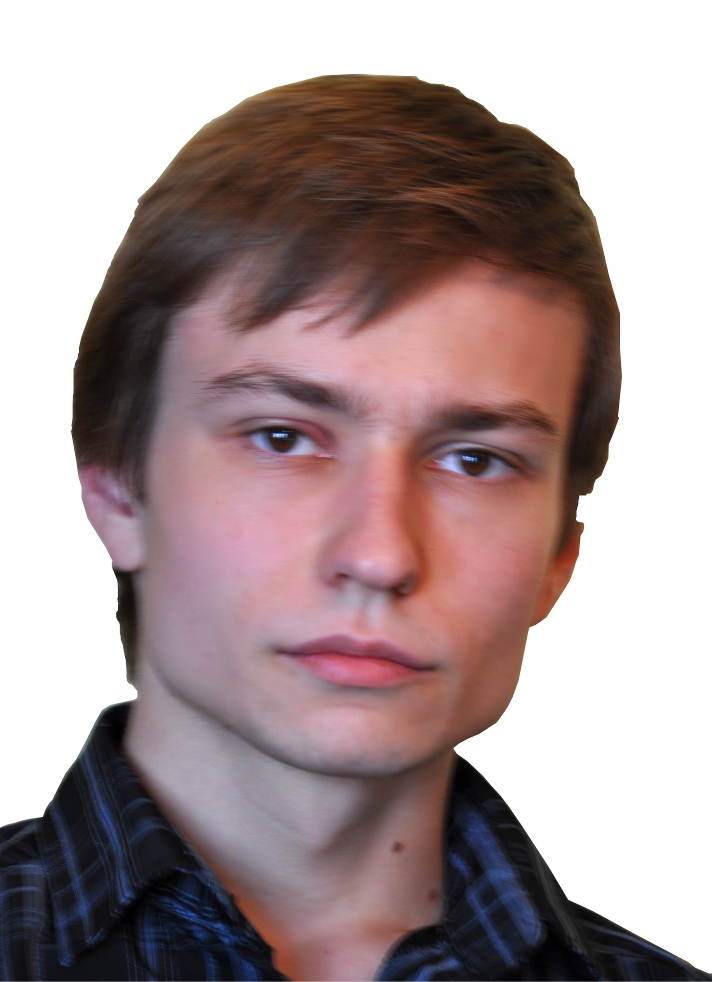
\includegraphics[width=120pt]{images/Martin_Osmera.jpg} &
                        \begin{tabular}{l}
                            Date of birth: 01/28/1988 \\
                            Place of birth: Brno, Czechoslovakia \\
                            Place of residence: Brno, Czech republic \\
                            Education: VUT FIT (university drop out)
                        \end{tabular}
                    \end{tabular}
                \end{table}
                \begin{dinglist}{73}
                    \setlength{\itemsep}{-3pt}
                    \item strong background in development for POSIX systems as a software developer in Siemens AG (2009-2012),
                    \item years of experience with pure programming as an open source software developer (mainly MCU 8051 IDE: 2006-2012),
                    \item experience with schematic and PCB design,
                    \item short experience with web page technologies (PHP, MySQL, (X)HTML, CSS, JavaScript, etc.)
                    \item operating systems: Linux (Gentoo, Ubuntu, Fedora, etc.), Windows (XP, 7), Unix (Solaris), BSD (FreeBSD)
                    \item 3 CCNA (Certified Cisco Network Associate) certificates (expired)
                    \item programming languages: C++, C, Assembler, Python, Tcl, Java, PHP, Bash, Perl, AWK ...
                    \item MCU (MicroController Unit) programming: AVR, PIC, MCS-51, Motorola HC11
                    \item other technologies: (X)HTML, LaTex, SQL, UML
                    \item other educations and/or certificates: Czech ``vyhláška 50 §5''
                    \item frameworks: Qt
                \end{dinglist}

            \subsubsection{Erik Chalupa}
                \begin{table}[h!]
                    \centering{}
                    \begin{tabular}{ll}
                        
\includegraphics[width=120pt]{images/Erik_Chalupa.jpg} &
                        \begin{tabular}{l}
                            Date of birth: 07/10/1991 \\
                            Place of birth: České Budějovice, Czechoslovakia \\
                            Place of residence: Šlapanice, Czech republic \\
                            Education: VUT FIT (university student)
                        \end{tabular}
                    \end{tabular}
                \end{table}
                \begin{dinglist}{73}
                    \setlength{\itemsep}{-3pt}
                    \item Programming languages: C++, C, Assembler, Java, Python, Perl, Bash, Pascal ...
                    \item frameworks: Qt, Swing
                    \item operating systems: Linux (Ubuntu, Fedora, OpenSuse), Windows (XP, 7), BSD (OpenBSD), Haiku OS
                    \item other technologies: HTML, LaTex, SQL, UML, VHDL
                    \item work experience: Symbian development
                    \item other educations and/or certificates: Czech ``vyhláška 50 §3''.
                \end{dinglist}

            \clearpage

            \subsubsection{Martin Madron}
                \begin{table}[h!]
                    \centering{}
                    \begin{tabular}{ll}
                        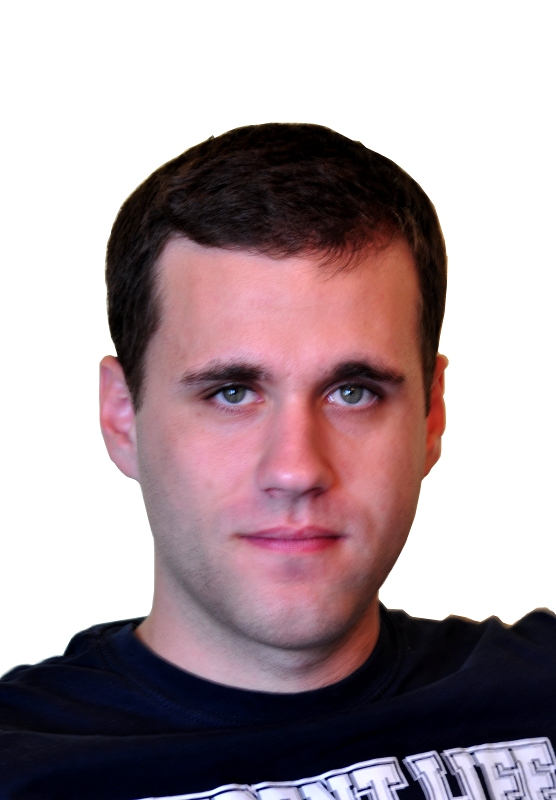
\includegraphics[width=120pt]{images/Martin_Madron.jpg} &
                        \begin{tabular}{l}
                            Date of birth: 07/29/1987 \\
                            Place of birth: Brno, Czechoslovakia \\
                            Place of residence: Prace, Czech republic \\
                            Education: VUT FEKT (Bc.)
                        \end{tabular}
                    \end{tabular}
                \end{table}
                \begin{dinglist}{73}
                    \setlength{\itemsep}{-3pt}
                    \item Programming languages: C, Assembler (AVR, MCS-51, PIC),
                    \item embedded system programming,
                    \item hardare definition languages: VHDL, Verilog,
                    \item experience with schematic and PCB design,
                    \item experience with PLC programming (DOMAT system, WAGO PLC)
                    \item experience with PSpice, Eagle, Matlab, AutoCAD, ...
                    \item electronics and Communication,
                    \item automation and Measurement,
                    \item power Electrical Engineering,
                    \item teleinformatics,
                    \item other educations and/or certificates: Czech ``vyhláška 50 §6''.
                \end{dinglist}

        \subsection{External}
            There will be also a few people who wouldn't be part of the core team itself but would participate on the project (web pages, accounting, law consulting, etc.)

\end{document}
